\documentclass[12pt, aspectratio=169]{beamer}

\usetheme{Madrid}
\usecolortheme{default}

% ───────────────── COLOR SETUP (ORANGE THEME) ─────────────────
\usepackage{xcolor}

\definecolor{mainorange}{RGB}{255, 140, 0}    % Dark Orange
\definecolor{softorange}{RGB}{255, 185, 80}   % Medium Orange
\definecolor{lightorange}{RGB}{255, 235, 205} % Blanched Almond

% Apply orange everywhere
\setbeamercolor{structure}{fg=mainorange}
\setbeamercolor{frametitle}{fg=white}
\setbeamercolor{title}{fg=white}

% Fix Madrid blue bars → orange
\setbeamercolor{palette primary}{bg=mainorange, fg=white}
\setbeamercolor{palette secondary}{bg=mainorange!85!black, fg=white}
\setbeamercolor{palette tertiary}{bg=mainorange!70!black, fg=white}

% Blocks
\setbeamercolor{block title}{bg=softorange, fg=black}
\setbeamercolor{block body}{bg=lightorange, fg=black}

% Bullets
\setbeamercolor{item}{fg=mainorange}

% Optional: remove navigation symbols
\setbeamertemplate{navigation symbols}{}

% ───────────────── PACKAGES ─────────────────
\usepackage{amsmath, amssymb}
\usepackage{tikz}
\usepackage{bm}
\usepackage{booktabs}
\usepackage{listings}

% ───────────────── LISTINGS CONFIGURATION ─────────────────
\lstset{
  basicstyle=\ttfamily\scriptsize,
  breaklines=true,
  frame=single,
  columns=fullflexible
}

% ───────────────── CUSTOM COLORS ─────────────────
\definecolor{highlightcol}{RGB}{220, 80, 0} % deep orange-red for emphasis
\definecolor{okgreen}{RGB}{0,130,60}

% ───────────────── FONTS ─────────────────
\setbeamerfont{frametitle}{series=\bfseries, size=\large}
\setbeamerfont{title}{series=\bfseries, size=\Large}
\setbeamerfont{subtitle}{series=\bfseries}

% ───────────────── CUSTOM COMMAND ─────────────────
% Changed \bm to \textbf to fix Overleaf table line-break swallowing issues
\newcommand{\res}[1]{\textcolor{highlightcol}{\textbf{#1}}}

\title{Single Machine Scheduling}
\subtitle{Minimizing Maximum Tardiness}
\author{CH. Taraka Abhinav - EE25BTECH11016}
\date{}

\begin{document}

% --- SLIDE 1 ---
\begin{frame}
    \titlepage
\end{frame}

% --- SLIDE 2 ---
\begin{frame}{1. The Problem Statement}
    \begin{block}{Question (2007 PI)}
        Four jobs have to be sequenced on a single facility, with the objective of minimizing the maximum tardiness: $\max_i |\text{Completion time}_i - \text{Due date}_i|$.
        
        \vspace{2mm}
        The jobs have due dates and processing times as follows:
        \begin{center}
            \small
            \begin{tabular}{c c c}
                \toprule
                \textbf{Job} & \textbf{Due date (days)} & \textbf{Processing time (days)} \tabularnewline
                \midrule
                P & 5 & 2 \tabularnewline
                Q & 6 & 10 \tabularnewline
                R & 3 & 3 \tabularnewline
                S & 7 & 4 \tabularnewline
                \bottomrule
            \end{tabular}
        \end{center}
        The last job that should be taken up is:

    
    \vspace{2mm}
    \begin{columns}
        \begin{column}{0.24\textwidth} \centering a) P \end{column}
        \begin{column}{0.24\textwidth} \centering b) Q \end{column}
        \begin{column}{0.24\textwidth} \centering c) R \end{column}
        \begin{column}{0.24\textwidth} \centering d) S \end{column}
    \end{columns}
    \end{block}
\end{frame}


% --- SLIDE 3 ---
\begin{frame}{2. Understanding the Concepts}
    \textbf{What are the variables?}
    \begin{itemize}
        \item \textbf{Processing Time ($p_i$):} How long it takes to finish the job.
        \item \textbf{Due Date ($d_i$):} The deadline promised to the customer.
        \item \textbf{Completion Time ($C_i$):} The actual day the job finishes.
    \end{itemize}
    
    \vspace{0.3cm}
    \begin{block}{What is Tardiness / Lateness?}
        Lateness is simply: $\text{Completion Time} - \text{Due Date}$ \quad ($C_i - d_i$). \\
        \vspace{0.1cm}
        If a job finishes \textit{after} its due date, it generates a penalty. Our goal is to arrange these jobs so that the \textbf{single worst delay} (Maximum Tardiness) is as small as physically possible.
    \end{block}
\end{frame}

% --- SLIDE 4 ---
\begin{frame}{3. Common Scheduling Rules}
    To sequence jobs on a single machine, we use standard dispatching rules:
    
    \vspace{0.3cm}
    \begin{itemize}
        \item \textbf{SPT (Shortest Processing Time):} Sort by smallest $p_i$. \\
        \textit{Objective:} Minimizes average completion time / flow time.
        \vspace{0.1cm}
        \item \textbf{LST (Least Slack Time):} Sort by smallest $(d_i - p_i)$. \\
        \textit{Objective:} Prioritizes jobs with the least buffer time.
        \vspace{0.1cm}
        \item \textbf{EDD (Earliest Due Date):} Sort by smallest $d_i$. \\
        \textit{Objective:} \res{Minimizes Maximum Tardiness ($T_{\max}$)}.
    \end{itemize}
    
    \vspace{0.3cm}
    \begin{block}{Which rule to choose?}
        Since our problem explicitly asks to minimize the \textbf{maximum tardiness}, we must use the \textbf{EDD Rule}.
    \end{block}
\end{frame}

% --- SLIDE 5 ---
\begin{frame}{4. Applying the EDD Rule}
    Let's extract the due dates from our original table and sort them from smallest (earliest) to largest (latest).
    
    \vspace{0.3cm}
    \begin{center}
    \renewcommand{\arraystretch}{1.3}
    \begin{tabular}{c c c c}
        \toprule
        \textbf{Original Job} & \textbf{Due Date ($d_i$)} & $\rightarrow$ & \textbf{Sorted Order (EDD)} \tabularnewline
        \midrule
        P & 5 & & \res{2nd} \tabularnewline
        Q & 6 & & \res{3rd} \tabularnewline
        R & \textbf{3} (Earliest) & & \res{1st} \tabularnewline
        S & 7 (Latest) & & \res{4th} \tabularnewline
        \bottomrule
    \end{tabular}
    \end{center}
    
    \vspace{0.3cm}
    Based purely on the EDD rule, the optimal processing sequence is: \\
    \begin{center}
        \Large \textbf{R $\rightarrow$ P $\rightarrow$ Q $\rightarrow$ S}
    \end{center}
\end{frame}

% --- SLIDE 6 ---
\begin{frame}{5. Verifying the Schedule (Proof)}
    Let's calculate the exact completion times to prove this works:
    
    \vspace{0.2cm}
    \begin{center}
    \renewcommand{\arraystretch}{1.2}
    \small
    \begin{tabular}{c c c c c}
        \toprule
        \textbf{Sequence} & \textbf{Proc. Time ($p_i$)} & \textbf{Completion Time ($C_i$)} & \textbf{Due Date} & \textbf{Tardiness ($|C_i - d_i|$)} \tabularnewline
        \midrule
        \textbf{1. Job R} & 3 & $0 + 3 = \textbf{3}$ & 3 & $\max(0, 3 - 3) = \res{0}$ \tabularnewline
        \textbf{2. Job P} & 2 & $3 + 2 = \textbf{5}$ & 5 & $\max(0, 5 - 5) = \res{0}$ \tabularnewline
        \textbf{3. Job Q} & 10 & $5 + 10 = \textbf{15}$ & 6 & $\max(0, 15 - 6) = \res{9}$ \tabularnewline
        \textbf{4. Job S} & 4 & $15 + 4 = \textbf{19}$ & 7 & $\max(0, 19 - 7) = \res{12}$ \tabularnewline
        \bottomrule
    \end{tabular}
    \end{center}
    
    \vspace{0.2cm}
    \begin{itemize}
        \item The maximum tardiness in this optimal sequence is 12 days.
        \item \textit{Note: If we placed Job Q last, Job Q would finish on Day 19 (Due Day 6), creating a worse maximum penalty of 13!}
    \end{itemize}
\end{frame}

% --- SLIDE 7 ---
\begin{frame}{6. Numerical Proof: What if we used SPT?}
    Let's test the \textbf{SPT (Shortest Processing Time)} rule, an intuitive alternative. We sort jobs by smallest $p_i$:
    
    \vspace{0.2cm}
    \textbf{SPT Sequence:} P (2) $\rightarrow$ R (3) $\rightarrow$ S (4) $\rightarrow$ Q (10)
    
    \vspace{0.2cm}
    \begin{center}
    \renewcommand{\arraystretch}{1.2}
    \small
    \begin{tabular}{c c c c c}
        \toprule
        \textbf{Sequence (SPT)} & \textbf{Proc. Time} & \textbf{Completion Time} & \textbf{Due Date} & \textbf{Tardiness} \tabularnewline
        \midrule
        \textbf{1. Job P} & 2 & $0 + 2 = \textbf{2}$ & 5 & $\max(0, 2 - 5) = \res{0}$ \tabularnewline
        \textbf{2. Job R} & 3 & $2 + 3 = \textbf{5}$ & 3 & $\max(0, 5 - 3) = \res{2}$ \tabularnewline
        \textbf{3. Job S} & 4 & $5 + 4 = \textbf{9}$ & 7 & $\max(0, 9 - 7) = \res{2}$ \tabularnewline
        \textbf{4. Job Q} & 10 & $9 + 10 = \textbf{19}$ & 6 & $\max(0, 19 - 6) = \res{13}$ \tabularnewline
        \bottomrule
    \end{tabular}
    \end{center}
    
    \vspace{0.2cm}
    \textbf{Result:} The maximum tardiness under SPT is \textbf{13 days} (caused by Job Q).
\end{frame}

% --- SLIDE 8 ---
\begin{frame}{7. Numerical Proof: What if we used LST?}
    Let's test the \textbf{LST (Least Slack Time)} rule. Slack = Due Date - Processing Time ($d_i - p_i$).
    
    \vspace{0.2cm}
    \textbf{Slack Calc:} P(5-2=3), Q(6-10=-4), R(3-3=0), S(7-4=3) \\
    \textbf{LST Sequence:} Q (-4) $\rightarrow$ R (0) $\rightarrow$ P (3) $\rightarrow$ S (3)
    
    \vspace{0.2cm}
    \begin{center}
    \renewcommand{\arraystretch}{1.2}
    \small
    \begin{tabular}{c c c c c}
        \toprule
        \textbf{Sequence (LST)} & \textbf{Proc. Time} & \textbf{Completion Time} & \textbf{Due Date} & \textbf{Tardiness} \tabularnewline
        \midrule
        \textbf{1. Job Q} & 10 & $0 + 10 = \textbf{10}$ & 6 & $\max(0, 10 - 6) = \res{4}$ \tabularnewline
        \textbf{2. Job R} & 3 & $10 + 3 = \textbf{13}$ & 3 & $\max(0, 13 - 3) = \res{10}$ \tabularnewline
        \textbf{3. Job P} & 2 & $13 + 2 = \textbf{15}$ & 5 & $\max(0, 15 - 5) = \res{10}$ \tabularnewline
        \textbf{4. Job S} & 4 & $15 + 4 = \textbf{19}$ & 7 & $\max(0, 19 - 7) = \res{12}$ \tabularnewline
        \bottomrule
    \end{tabular}
    \end{center}
    
    \vspace{0.2cm}
    \textbf{Result:} The maximum tardiness is \textbf{12 days}, but notice that \textit{every single job} is penalized!
\end{frame}

% --- SLIDE 9 ---
\begin{frame}{8. Comparison: EDD vs SPT vs LST}
    \begin{table}[]
        \centering
        \renewcommand{\arraystretch}{1.3}
        \begin{tabular}{l c c}
            \toprule
            \textbf{Rule \& Sequence} & \textbf{Tardiness Profile} & \textbf{Max Tardiness ($T_{\max}$)} \tabularnewline
            \midrule
            \textbf{EDD} (R-P-Q-S) & \{0, 0, 9, \res{12}\} & \textbf{12} (Optimal) \tabularnewline
            \textbf{SPT} (P-R-S-Q) & \{0, 2, 2, \res{13}\} & \textbf{13} \tabularnewline
            \textbf{LST} (Q-R-P-S) & \{4, 10, 10, \res{12}\} & \textbf{12} \tabularnewline
            \bottomrule
        \end{tabular}
    \end{table}
    
    \vspace{0.3cm}
    \textbf{Conclusion:} 
    \begin{itemize}
        \item \textbf{SPT} pushes the long job (Q) to the end, causing a peak penalty spike of 13.
        \item \textbf{LST} ties the peak penalty of 12, but creates a \textit{cascading delay} where all jobs are severely late (Sum of penalties = 36 vs EDD's 21).
        \item \textbf{EDD} mathematically guarantees the lowest possible maximum penalty while ensuring early jobs finish on time!
    \end{itemize}
\end{frame}

% --- SLIDE 10 ---
\begin{frame}{Final Conclusion}
    The problem asks for the \textbf{last job} that should be taken up in the optimal sequence.
    
    \vspace{0.5cm}
    \begin{block}{Optimal Sequence Result}
        \centering
        \Large \textbf{R $\rightarrow$ P $\rightarrow$ Q $\rightarrow$ \res{S}}
    \end{block}
    
    \vspace{0.5cm}
    The last job in the sequence is \textbf{Job S}.
    
    \vspace{0.5cm}
    \textbf{Correct Option:} \textcolor{okgreen}{\textbf{(d) S}}
\end{frame}

\begin{frame}[fragile]{Python: Data Setup \& Analysis}
\begin{lstlisting}
import matplotlib.pyplot as plt
import numpy as np

# Job Data
jobs = {
    'P': {'p': 2, 'd': 5},
    'Q': {'p': 10, 'd': 6},
    'R': {'p': 3, 'd': 3},
    'S': {'p': 4, 'd': 7}
}

# Sequences
seq_edd = ['R', 'P', 'Q', 'S']
seq_spt = ['P', 'R', 'S', 'Q']
seq_lst = ['Q', 'R', 'S', 'P']

def analyze_sequence(seq):
    current_time = 0
    gantt = []
    abs_lateness = {}
    actual_lateness = {}
    cumulative_times = [0]
\end{lstlisting}
\end{frame}
\begin{frame}[fragile]{Python: Data Setup \& Analysis}
\begin{lstlisting}
    for job in seq:
        p = jobs[job]['p']
        d = jobs[job]['d']
        start = current_time
        current_time += p

        gantt.append((job, start, p, d))
        abs_lateness[job] = abs(current_time - d)
        actual_lateness[job] = current_time - d
        cumulative_times.append(current_time)

    return gantt, abs_lateness, actual_lateness, cumulative_times
\end{lstlisting}
\end{frame}

\begin{frame}[fragile]{Python: Gantt Chart Generation}
\begin{lstlisting}
gantt_edd, _, _, _ = analyze_sequence(seq_edd)
gantt_spt, _, _, _ = analyze_sequence(seq_spt)
gantt_lst, _, _, _ = analyze_sequence(seq_lst)

colors = {'P': '#2ca02c', 'Q': '#d62728',
          'R': '#1f77b4', 'S': '#ff7f0e'}

fig1, ax1 = plt.subplots(figsize=(12, 8))

def draw_gantt_row(ax, gantt_data, y_base):
    for job, start, p, d in gantt_data:
        ax.broken_barh([(start, p)], (y_base, 6))
        ax.text(start + p/2, y_base + 3, job)

draw_gantt_row(ax1, gantt_lst, 5)
draw_gantt_row(ax1, gantt_spt, 20)
draw_gantt_row(ax1, gantt_edd, 35)

plt.savefig("G.png")
\end{lstlisting}
\end{frame}

\begin{frame}{Gantt Chart Comparison}
\centering

\includegraphics[width=0.75\linewidth]{figs/G.png}

\vspace{0.3cm}
\textbf{Observation:}
\begin{itemize}
    \item EDD gives minimum maximum lateness
    \item Clear visualization of scheduling impact
\end{itemize}
\end{frame}

\begin{frame}[fragile]{Python: Absolute Deviation}
\begin{lstlisting}
job_labels = ['P', 'Q', 'R', 'S']
x = np.arange(len(job_labels))
width = 0.25

_, abs_lat_edd, _, _ = analyze_sequence(seq_edd)
_, abs_lat_spt, _, _ = analyze_sequence(seq_spt)
_, abs_lat_lst, _, _ = analyze_sequence(seq_lst)

edd_vals = [abs_lat_edd[j] for j in job_labels]
spt_vals = [abs_lat_spt[j] for j in job_labels]
lst_vals = [abs_lat_lst[j] for j in job_labels]

fig2, ax2 = plt.subplots()
ax2.bar(x - width, edd_vals, width, label='EDD')
ax2.bar(x, spt_vals, width, label='SPT')
ax2.bar(x + width, lst_vals, width, label='LST')

plt.savefig("A.png")
\end{lstlisting}
\end{frame}

\begin{frame}{Absolute Deviation Plot}
\centering
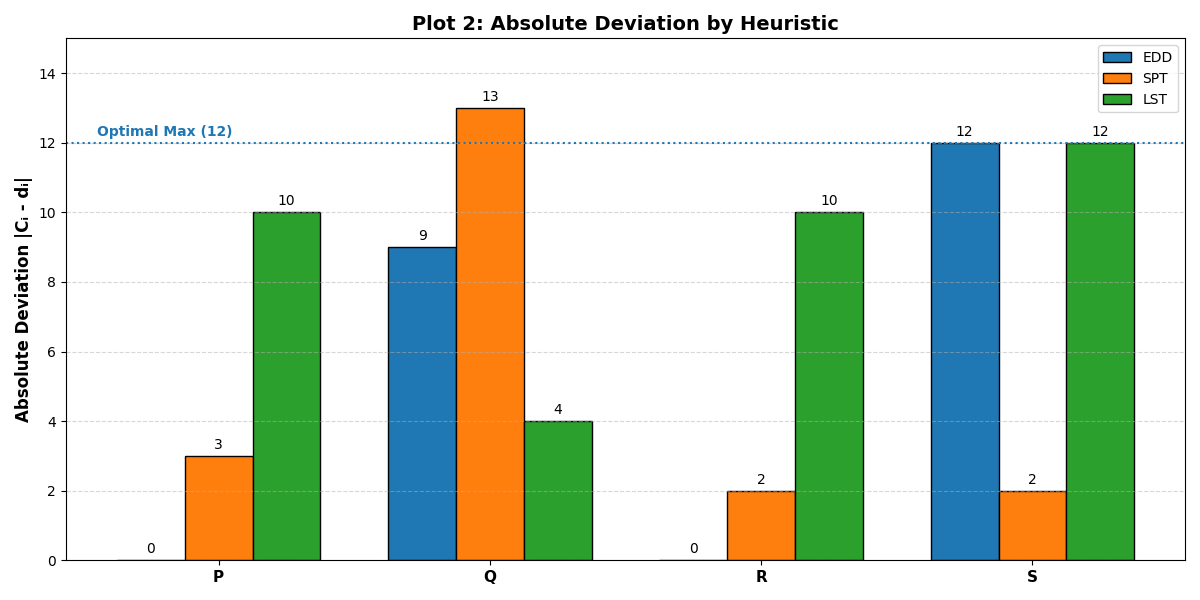
\includegraphics[width=0.85\linewidth]{figs/A.png}
\end{frame}

\begin{frame}[fragile]{Python: Completion Time Trajectory}
\begin{lstlisting}
_, _, _, cum_edd = analyze_sequence(seq_edd)
_, _, _, cum_spt = analyze_sequence(seq_spt)
_, _, _, cum_lst = analyze_sequence(seq_lst)

steps = [0, 1, 2, 3, 4]

fig4, ax4 = plt.subplots()
ax4.step(steps, cum_edd, label='EDD', where='post')
ax4.step(steps, cum_spt, label='SPT', where='post')
ax4.step(steps, cum_lst, label='LST', where='post')

ax4.legend()
plt.savefig("T.png")
\end{lstlisting}
\end{frame}

\begin{frame}{Completion Time Trajectory}
\centering
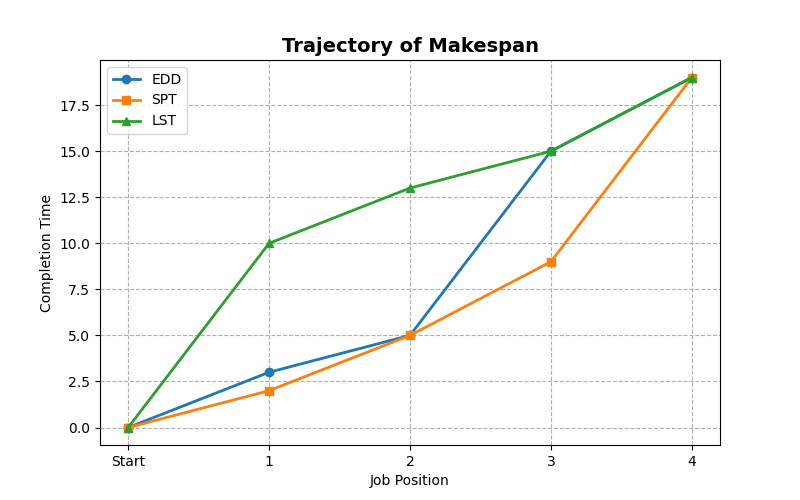
\includegraphics[width=0.85\linewidth]{figs/T.png}
\end{frame}

\end{document}